\section{Results and Discussion}\label{sec:Discussion}
\subsection{Sampling of States using Metropolis}

\begin{figure}
	\begin{subfigure}{\textwidth}
		\centering
		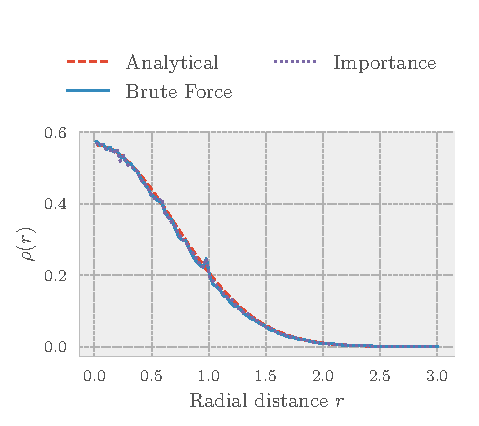
\includegraphics[width=.8\linewidth]{figures/density1.pdf}
		\subcaption{Approximation of onebody density using Metropolis brute force sampling vs analytical(kilde)}
		\label{fig:sfig1}
	\end{subfigure}%
	\begin{subfigure}{\textwidth}
		\centering
		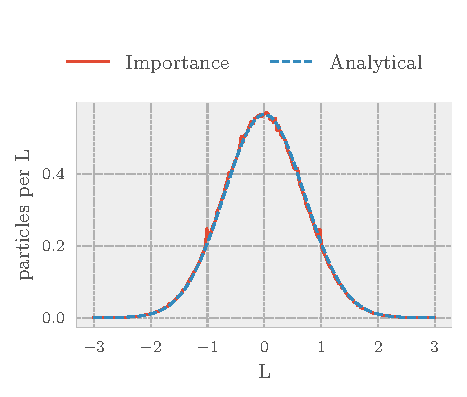
\includegraphics[width=.8\linewidth]{figures/density2.pdf}
		\subcaption{Approximation of onebody density using Metropolis importance sampling vs analytical}
		\label{fig:sfig2}
	\end{subfigure}
	\caption{One-body density of 1 boson in 1 dimmension, using $N = 1e6$ cycles, $\omega = 1$, $\alpha = 0.5$.}
	\label{fig:1 part 1 dim density}
\end{figure}

\begin{figure}
	\begin{subfigure}{\textwidth}
		\centering
		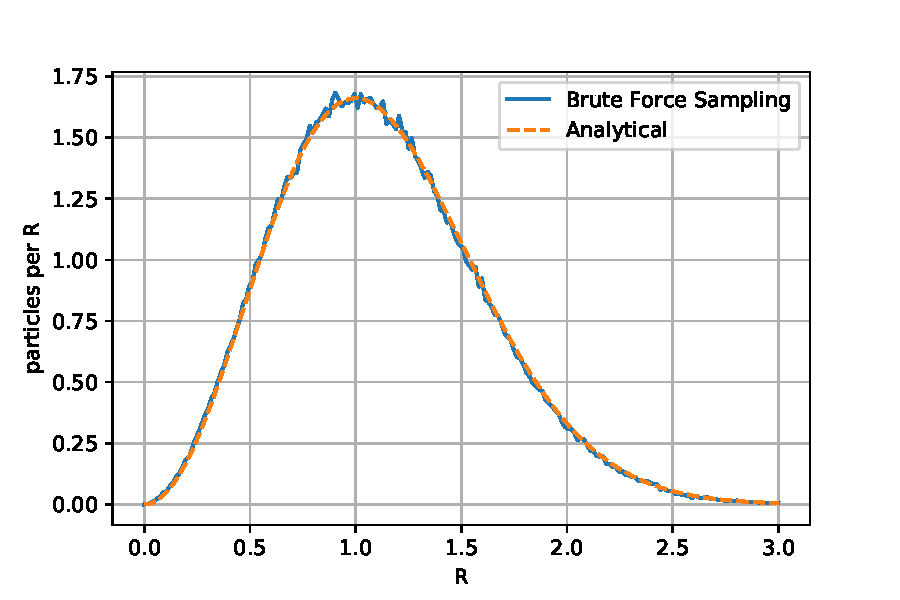
\includegraphics[width=.8\linewidth]{figures/density3.pdf}
		\subcaption{Approximation of radial onebody density using Metropolis brute force sampling vs analytical}
		\label{fig:sfig1}
	\end{subfigure}%
	\begin{subfigure}{\textwidth}
		\centering
		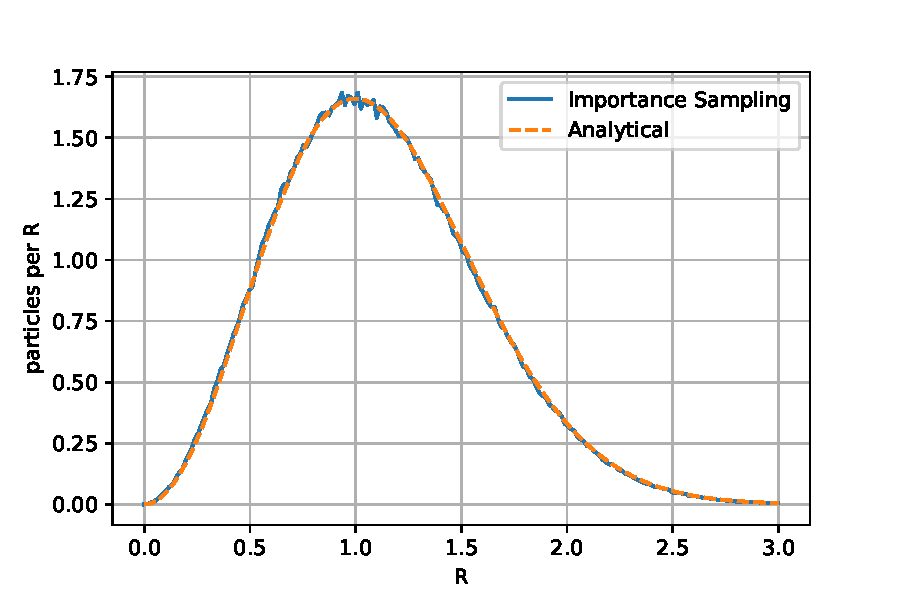
\includegraphics[width=.8\linewidth]{figures/density4.pdf}
		\subcaption{Approximation of radial onebody density using Metropolis importance sampling vs analytical}
		\label{fig:sfig2}
	\end{subfigure}
	\caption{Radial one-body density of 2 non-interacting bosons in 3 dimmensions, using $N = 1e6$ cycles, $\omega = 1$, $\alpha = 0.5$.}
	\label{fig:2 part 3 dim density}
\end{figure}

In \autoref{fig:1 part 1 dim density}  we see that both brute force sampling and importance sampling manage to approximate the onebody density derived from the non-interacting trial wave function: Aside from the statistical noise introduced by the finite number of Monte-Carlo cycles, the approximated densities follow the analytical result closely. Figure \autoref{fig:2 part 3 dim density} demonstrates that this also scales to more particles and dimensions, as seen from the radial onebody density of two particles in three dimensions. 


\subsection{Blocking of Local Energy}
\begin{figure}
	\begin{subfigure}{\textwidth}
		\centering
		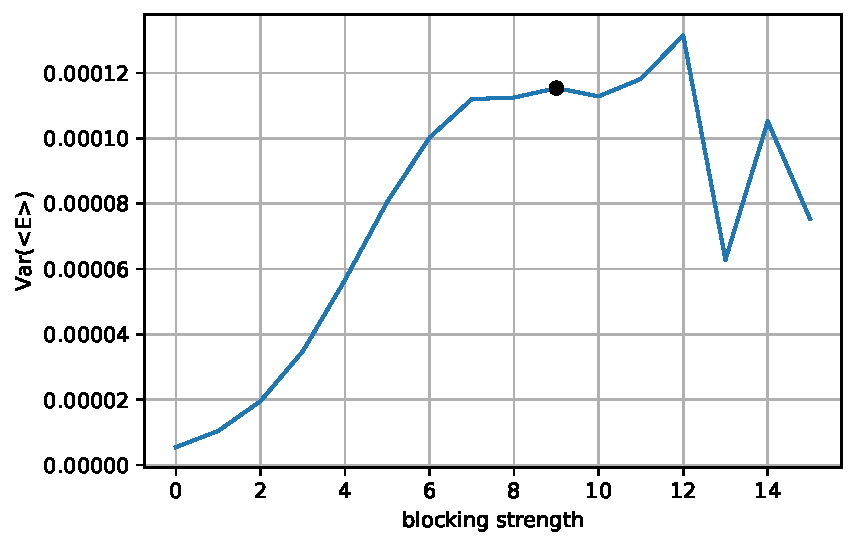
\includegraphics[width=.8\linewidth]{figures/blocking1.pdf}
		\subcaption{Brute Force Sampling}
	\end{subfigure}%
	\begin{subfigure}{\textwidth}
		\centering
		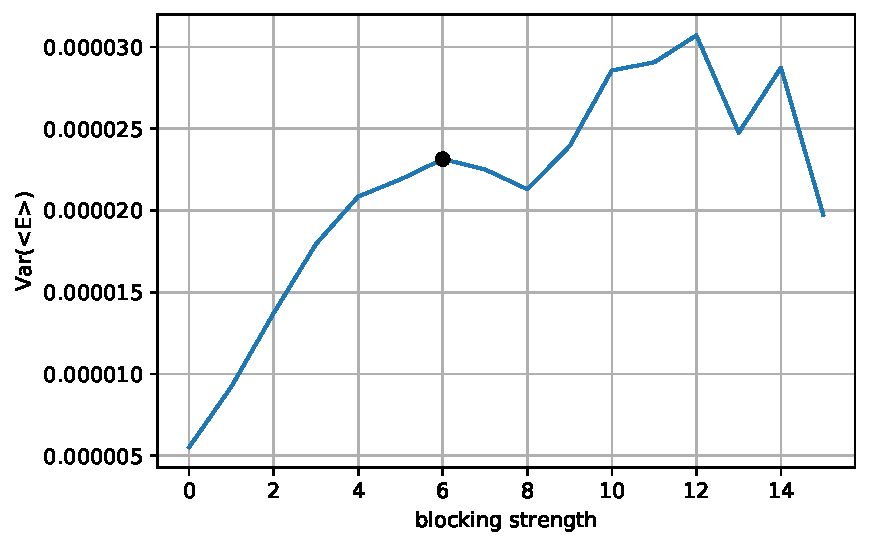
\includegraphics[width=.8\linewidth]{figures/blocking2.pdf}
		\subcaption{Importance Sampling}
	\end{subfigure}%
	\centering
	\caption{Variance of the estimate of $<E>$ using blocked values of local energy at various strengths. The data has been produced for 40 non-interacting bosons i 3 dimension, using $N = 2^{20}$ cycles, $\alpha = 0.8$, $\omega = 1$, with and without importance sampling}
	\label{fig:blocking1}
\end{figure}

In \autoref{fig:blocking1}, we see the effect of applying blocking on the local energy data before calculating the variance of the estimator (kilde). Although the local energies are sampled from an approximately correct distribution, as indicated by \autoref{fig:2 part 3 dim density}, the data is produced by moving a single electron at a time. Moreover, the move may even be rejected by the metropolis algorithm. Because of this, the data is highly correlated, causing an underestimation of the variance as seen for the unblocked data(blocking strength $0$). After repeated blocking, the variance stabilizes when the data is approximately uncorrelated. Note that this happens at different strengths of blocking for brute force sampling and importance sampling. This indicates that latter method creates data that are less correlated. This makes sense, as importance sampling uses additional information from the wave function and explores the space of states more efficiently than brute force. \autoref{fig:blocking1} shows that the variance stabilizes at strength $6$ when using importance sampling, as opposed to $9$ when using brute force. This grants us 8 times the effective amount of data and thus a smaller variance of the estimator.

\begin{figure}
	\centering
	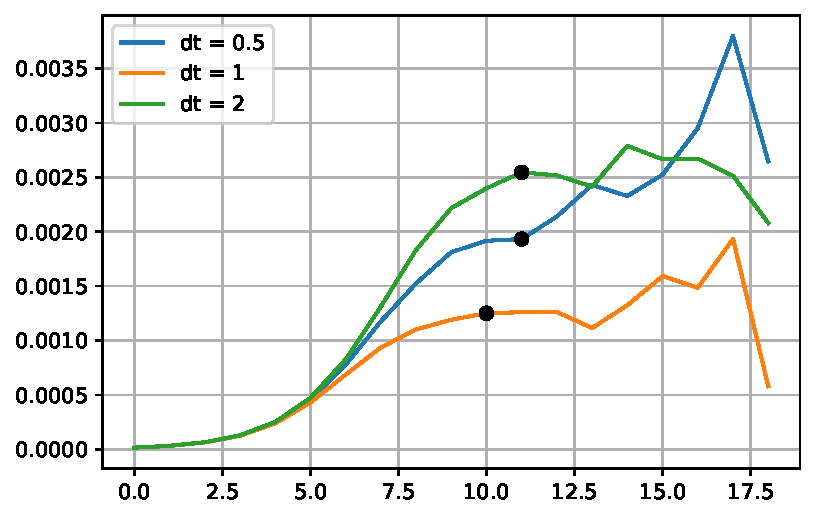
\includegraphics[width=.8\linewidth]{figures/blocking3.pdf}
	\caption{Variance of the estimate of $<E>$ using blocked values of local energy at various strengths. The data has been produced for 40 non-interacting bosons i 3 dimension, using $N = 2^{20}$ cycles, $\alpha = 0.8$, $\omega = 1$, using importance sampling with step length $0.5$, $1$ and $2$, respectively}
	\label{fig:blocking2}
\end{figure}

\begin{table}[t]
	\begin{tabular}{lclclclc}
		\hline
		\hline
		dt & \langle E \rangle & blocking strength$\\
		\hline
		0.5 & 68.009 \pm 0.044 & 11\\
		1 & 68.039 \pm 0.035 & 10\\
		2 & 67.942 \pm 0.050 & 11\\
		\hline
	\end{tabular}
	\caption{Estimate of energy $\langle E \rangle$ for 40 particles, $\alpha = 0.3$, $\omega = 1$}
	\label{tab:blocking}
\end{table}

\autoref{fig:blocking2} repeats the results of \autoref{fig:blocking1}, but for a larger system of $40$ non-interacting bosons using importance sampling only. Step lengths of $0.5$, $1$ and $2$ was used. For a larger system, the local energies will tend to become more correlated as the moving of a single particle becomes a comparatively small change. This can be seen from the figure, as a higher order of blocking is required to stabilize the variance than in the two particle case.

Further, the least correlated data was produces for step length $\delta t = 1$, requiring blocking strength $10$ as opposed to $11$ for $\delta t = 0.5$ and $2$. Using a step length too small results in the local energy changing minimally from cycle to cycle, increasing the correlation and minimizing the effective amount of data. The same happens if the step length is too big, as drastic moves will tend to be rejected often, causing repeated values to be sampled. \autoref{tab:blocking} presents the resulting estimates of energy with the uncertainty established using the blocking. This shows that the estimated energy is only sensitive to the step length in the sense that more cycles may be needed to get an accurate result of the step length is taken too small or too big.
 
\subsection{Energy of Non-Interacting System}
\begin{figure}
	\begin{subfigure}{\textwidth}
		\centering
		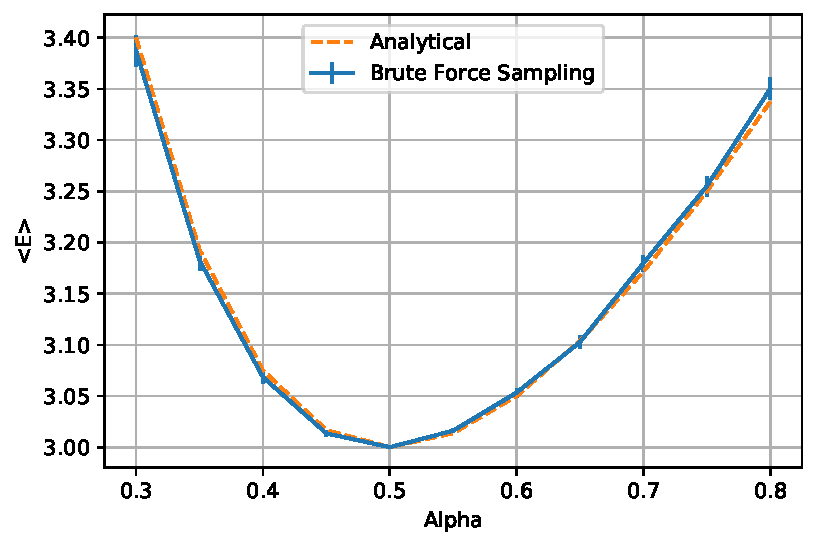
\includegraphics[width=.8\linewidth]{figures/energy_bruteforce1.pdf}
		\subcaption{Estimate of $\langle E \rangle$}
	\end{subfigure}%
	\begin{subfigure}{\textwidth}
		\centering
		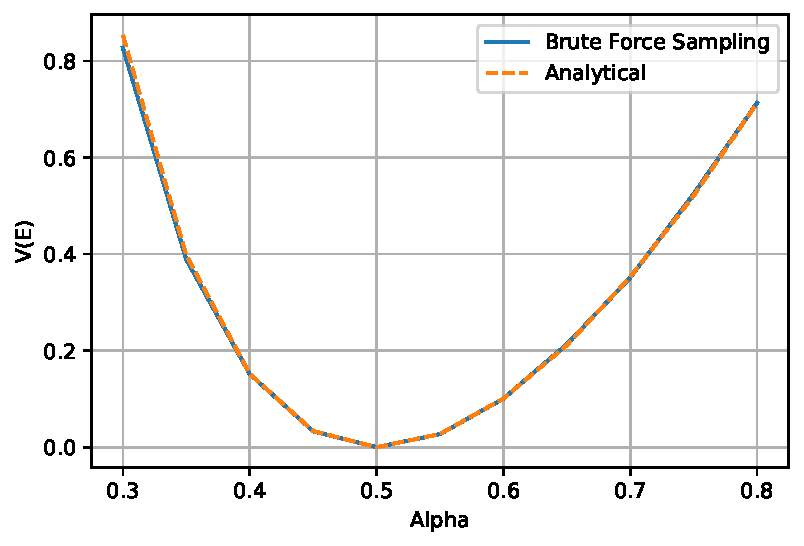
\includegraphics[width=.8\linewidth]{figures/variance_bruteforce1.pdf}
		\subcaption{Estimate of $V(E)$}
	\end{subfigure}%
	\centering
	\caption{Estimated energy $\langle E \rangle$ and variance $V(E)$ for two non-interacting bosons, using $2^{17}$ cycles, $\omega = 1$ and brute force sampling. Errorbars was established using blocking. Teh analytical result is plotted for comparison. }
	\label{fig:brute force energy}
\end{figure}

As seen from \autoref{fig:brute force energy}, the estimated energy is consistent with the analytical within the uncertainty obtained using blocking. For $\alpha = 0.5$, the estimated value coincide with the analytical without any uncertainty, and $V(E)$ becomes zero. This is expected, as our trial wave function becomes the exact solution for $\alpha = 0.5$ for the non-interacting system.  

\begin{figure}
	\begin{subfigure}{\textwidth}
		\centering
		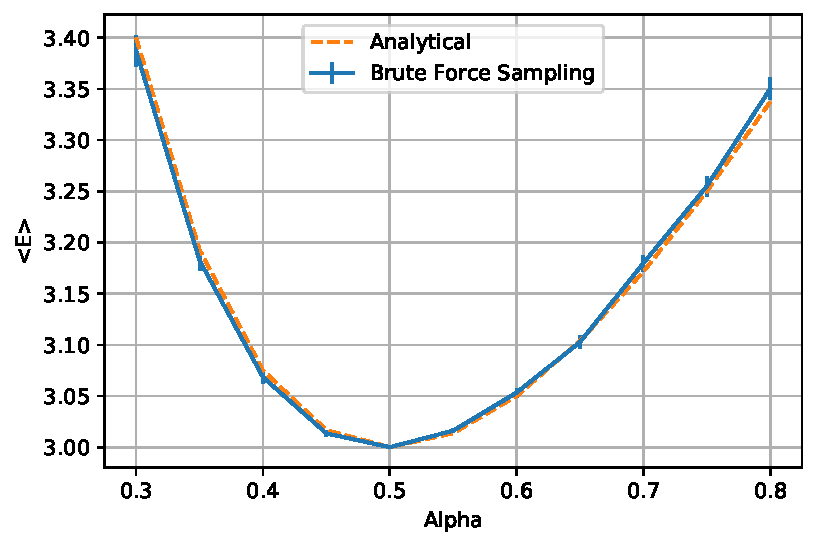
\includegraphics[width=.8\linewidth]{figures/energy_bruteforce1.pdf}
		\subcaption{Estimate of $\langle E \rangle$}
	\end{subfigure}%
	\begin{subfigure}{\textwidth}
		\centering
		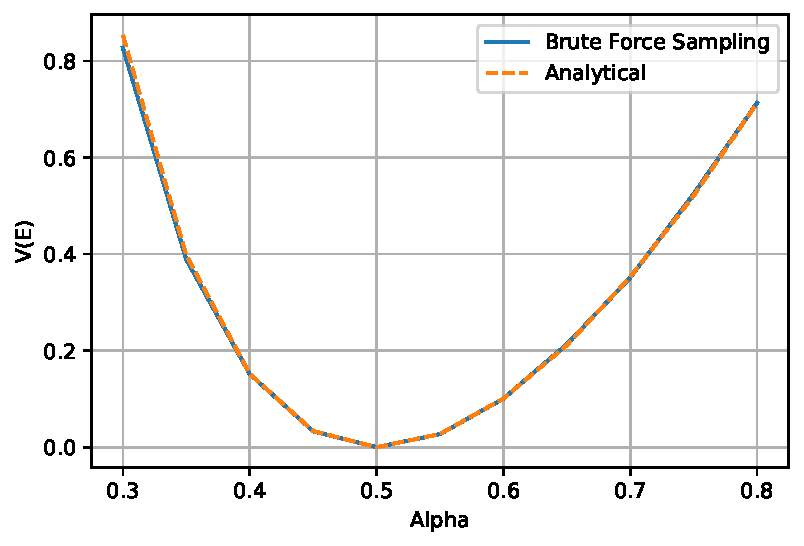
\includegraphics[width=.8\linewidth]{figures/variance_bruteforce1.pdf}
		\subcaption{Estimate of $V(E)$}
	\end{subfigure}%
	\centering
	\caption{Estimated energy $\langle E \rangle$ and variance $V(E)$ for two non-interacting bosons, using $2^{17}$ cycles, $\omega = 1$ and importance sampling. Errorbars was established using blocking. The analytical result is plotted for comparison. }
	\label{fig:importance energy}
\end{figure}

\autoref{fig:importance energy} presents the same data as \autoref{fig:brute force energy}, but using importance sampling. The data is consistent with the previous discussion, showing that importance sampling reproduces the correct results with respect to the estimation of the energy.

\subsection{Numerical and Analytical Laplacian}
\begin{figure}
	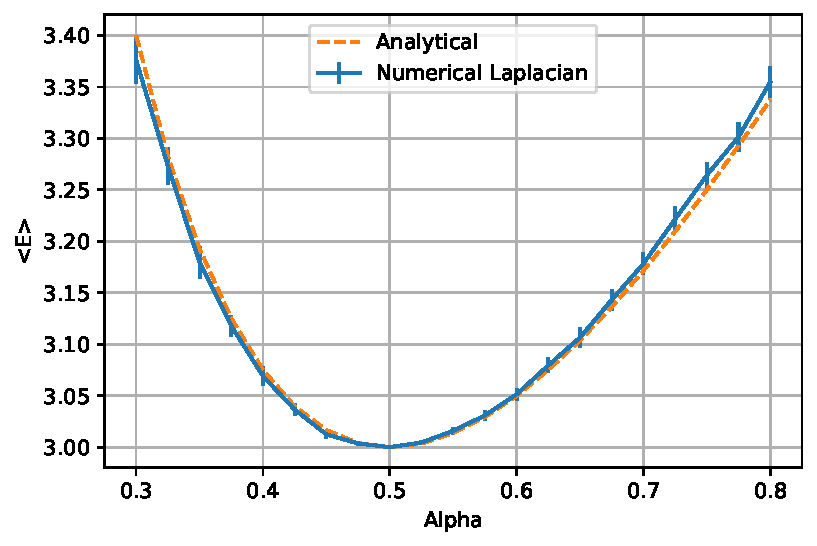
\includegraphics[width=.8\linewidth]{figures/numericalLap.pdf}
	\centering
	\caption{Estimated energy $\langle E \rangle$ for two non-interacting bosons, using numerically evaluated laplacian, $2^{17}$ cycles, $\omega = 1$ and importance sampling. Errorbars was established using blocking. }
	\label{fig:numerical lap}
\end{figure}

\begin{figure}
	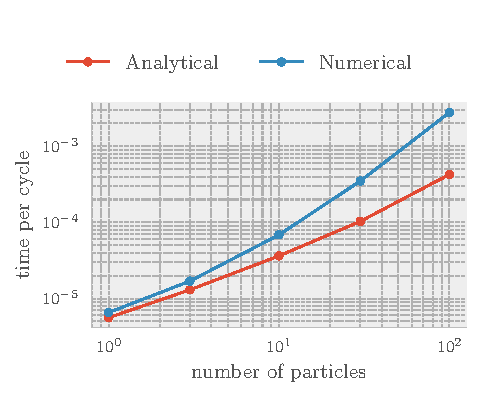
\includegraphics[width=.8\linewidth]{figures/numericalTime.pdf}
	\centering
	\caption{Comparison of CPU-time of numerical and analytical laplacian for different numbers of particles. The timing is with respect to the whole simulation, including writing to file}
	\label{fig:numerical time}
\end{figure}

Yet again, \autoref{fig:numerical lap} repeats the analysis of \autoref{fig:brute force energy} and 
\autoref{fig:importance energy}, but using finite difference for evaluating the Laplacian of the wave function rather than the analytical expression. The resulting estimate is within the statistical error of the Monte-Carlo simulation, showing that finite difference implementation is stable and of sufficient accuracy. 

\autoref{fig:numerical time} demonstrates that the CPU-time when using the analytical Laplacian is smaller than when using the finite difference method, for $1$ to $30$ non-interacting bosons. However, the speedup is small and hard to quantify, and even more negligible for systems of more particles. This is perhaps because, ultimately, in realistic simulations, a great portion of the CPU-time goes to other tasks such as writing the positions to file. The increase in CPU-time because of the numerical evaluation is not so big in comparison.    
\subsection{Interacting Potentials}
\begin{figure}
	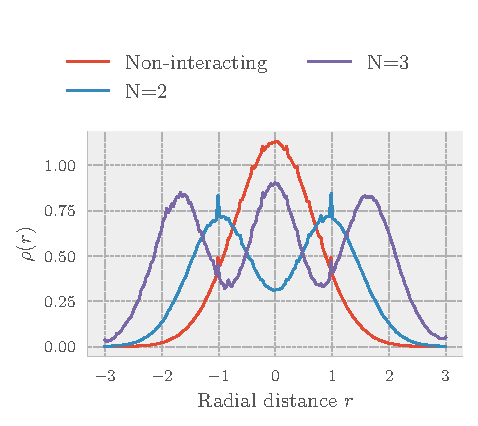
\includegraphics[width=.8\linewidth]{figures/interactingDensity.pdf}
	\centering
	\caption{One body density in one dimension, for two non-interacting bosons, two interacting bosons, and three interacting bosons. $N = 400000$, $\alpha = 0.5$, $\omega = 1$, $a = 1$. The densities are compared to the analytical one body density for two non-interacting bosons.}
	\label{fig:interacting density}
\end{figure}

\autoref{interacting density} presents the 1 dimmensional onebody density for two non-interacting bosons, two interacting bosons of radius $a = 1$, and three interacting bosons of the same radius. 
For the non-interacting case, the interacting model was used to produce the samples with the hard shell radius set to $a = 0$. Comparing it to the analytical result, we see that the implementation is consistent with the non-interacting case. For $a=1$, we see that the correlating term produces a repulsive effect, creating two distinct maxima of relatively higher density. For the case of three interacting bosons, we instead get three maxima. Intuitively, repelling particles seek to maximize the distance from eachother, while still being confined by the harmonic potential.

\subsection{Optimal Parameter \(\alpha\)}
\begin{figure}
	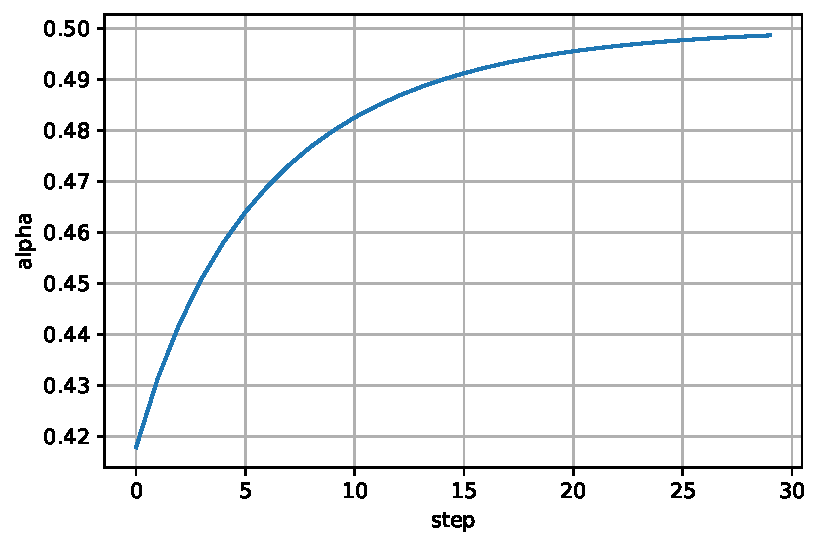
\includegraphics[width=.8\linewidth]{figures/gd.pdf}
	\centering
	\caption{Gradient decent on the parameter $\alpha$ for two non-interacting bosons, learning rate $\mu = 0.01$, $N = 10000$ steps and $\omega = 1$}
	\label{fig:gd}
\end{figure}

\autoref{fig:gd} shows the result of gradient descent used to minimize the estimated energy $\langle E \rangle$ with respect to $\alpha$. For the non-interacting case, the method converges to $\alpha = 0.5$, which we know to be the analytical value for the exact wave function. This establish confidence that the method of gradient decent also yields the optimal $\alpha$ for the interacting case, where a analytical solution is not known. 

\subsection{Interacting Bosons in Elliptical Potential}

\begin{table}[t]
	\begin{tabular}{lclclclc}
		\hline
		\hline
		Bosons & \langle E \rangle & optimal $\alpha$\\
		\hline
		10 & 24.3985 \pm 0.0011 & 0.49752\\
		50 & 127.37 \pm 0.035 & 0.48903\\
		100 & 265.69 \pm 0.27 & 0.48160\\
		\hline
	\end{tabular}
	\caption{Estimate of energy $\langle E \rangle$ for 10, 50 and 100 particles in elliptical potential. $\beta = \gamma = 2.8284$. $N = 2^20$ cycles per thread, of $12$ threads. Importance sampling with a step length $0.5$ was used. Gradient decent was used to optimize $\alpha$}
	\label{tab:energies}
\end{table}

\begin{figure}
	\begin{subfigure}{\textwidth}
		\centering
		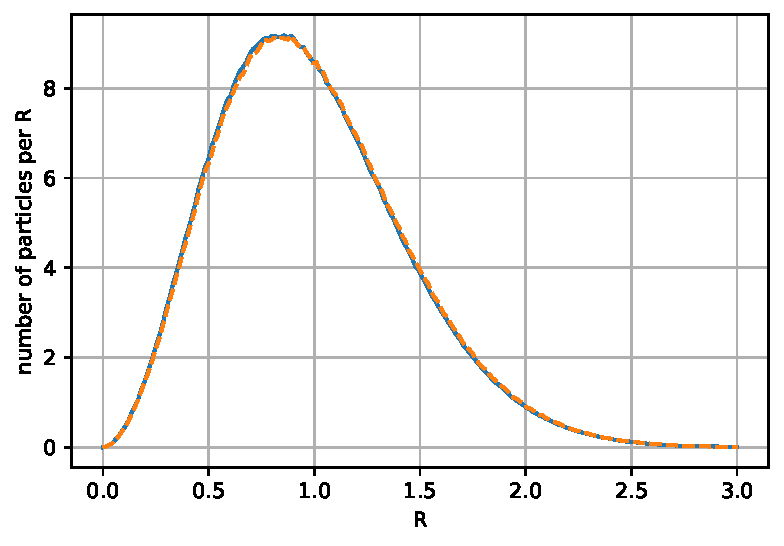
\includegraphics[width=.8\linewidth]{figures/density10.pdf}
		\subcaption{Radial onebody density for $10$ bosons in elliptical trap, interacting and non-interacting case}
	\end{subfigure}%
	\begin{subfigure}{\textwidth}
		\centering
		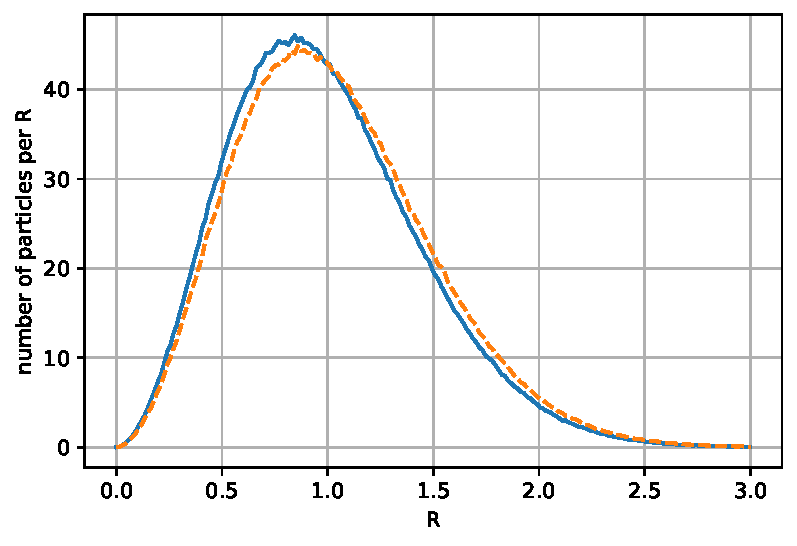
\includegraphics[width=.8\linewidth]{figures/density50.pdf}
		\subcaption{Radial onebody density for $50$ bosons in elliptical trap, interacting and non-interacting case}
	\end{subfigure}%
	\begin{subfigure}{\textwidth}
		\centering
		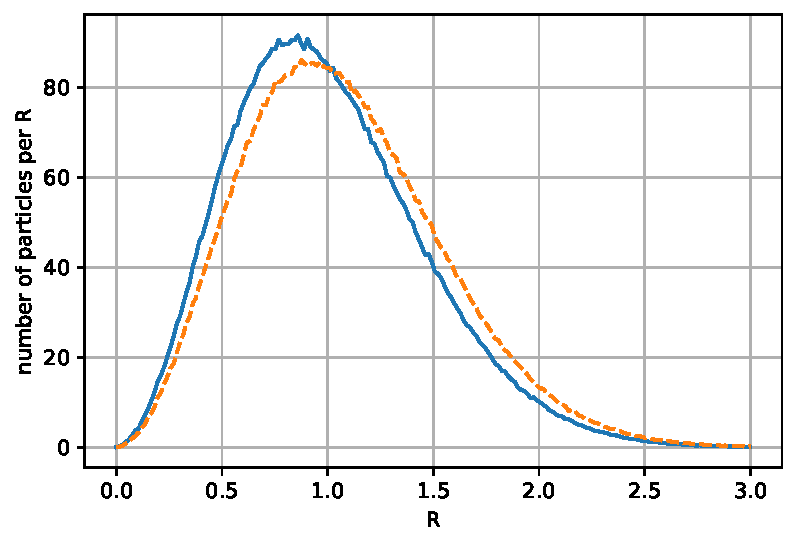
\includegraphics[width=.8\linewidth]{figures/density100.pdf}
		\subcaption{Radial onebody density for $100$ bosons in elliptical trap, interacting and non-interacting case}
	\end{subfigure}%
	\centering
	\caption{Comparison of the radial onebody density for interacting and non-interacting bosons. The hardshell radius of in the interacting case is $a = 0.0043$. The elliptical potential is defined by $\beta = \gamma =  2.82843$. }
	\label{fig:ellipticalOnebodyDensity}
\end{figure}

\autoref{tab:energies} presents the estimated ground state energies for $10$, $50$ and $100$ interacting bosons confined by a elliptical potential. The optimal value for $\alpha$ was found using gradient decent. Notice that the optimal value is decreasing with the number of particles in the interacting case, whereas it is analytically $\alpha = 0.5$ in the non-interacting case for any number of particles. A smaller value of $\alpha$ indicates the onebody exponential functions widens, resulting in a wider distribution of particles. This makes sense, as hardshell bosons interact repulsively. Therefore, the more particles, the more energetically favorable is it to spread out. This is consistent with the 1D result presented in \autoref{fig:ellipticalOnebodyDensity}. As the number of particles increase, the radial onebody density tends to migrate outward with respect to the non-interacting system. 

The ground state energy was most accurately calculated for $10$ bosons. This is because, as discussed earlier, data tend to be less correlated for smaller systems. To get a accurat estimate for larger systems, a increase in the number of cycles is appropriate. However, because of limited computer power, this was neglected. 

A comment on the interpretation of the error presented in \autoref{tab:energies} is appropriate:
The error is an estimate of the statistical error in the estimated ground state energy introduced by the Monte-Carlo simulation. It does not account for possible error introduced in the estimation of $\alpha$ that minimizes the energy. This is much harder to quantity, and is possibly large in the case for $50$ and $100$ particles, as the gradient was hard to estimate consistently. Furthermore, the error does not in any way establish a confidence interval for the true ground state value of the Hamiltonian we are investigating, which is harder still to quantify. Our estimate a approximate minimum only in the subspace spanned by out trial wave function, which is hopefully, somewhat close the exact solution of the system.






